\chapter{Requirements Analysis}\label{C:ra}
The design of the visualisation was based heavily on User Centered Design as it provided a method of user interface design as well as visualisation design. User Centered Design is a process in which the needs, wants, and limitatons of the end users of a system are given extensive attention. To achieve this it meant that personas were created, which are an archetype personification of a set of related users representing the needs of larger groups of users. These personas act as stand-ins for real users and describes them in terms of their goals and personal characteristics and although they personas are fictitious, they are based on knowledge of real users. This design methodology supported my understanding of how users were likely to use the visualisation produced and also provided clear defined personas that could be validated during evaluation of the visualistaion with real users that match the core values of the personas.
\\\\

\section{User models}
Below are the three personas that were used in the design of the visualisation for this project. They depict users that would use the visualisation in the context of a terminal or display in an observatory environment. 
\subsection{John Truman (Primary Persona)}\
24 year old John is interested in planets and space and has a basic knowledge about both. John has used is used to playing computer games and using visualisations and is not overwhelmed understanding and using new systems. He finds that he learns better when provided with visual examples than when reading or listening to information. John is comfortable using keyboard and mouse when interacting with a computer but is also happy to use other gesture based methods. 
\subsection{Cara Thompson (Secondary Persona)}
\subsection{Rob Adams (Secondary Persona)}

\section{Scenarios}

\section{Requirements summary}

\section{Existing systems}
\subsection{Worlds: The Kepler Planet Candidates - Non Interactive}
 This animation \cite{worlds} shows  planet candidates found by NASA's Kepler mission. These candidates are animated in orbit around a single star. They are drawn to scale with accurate radii, orbital periods, and orbital distances. They range in size from 1/3 to 84 times the radius of Earth. Colors represent an estimate of temperature with red indicating warmest, and blue indicating coldest candidates. 
\begin{figure}[h!]
  \centering
      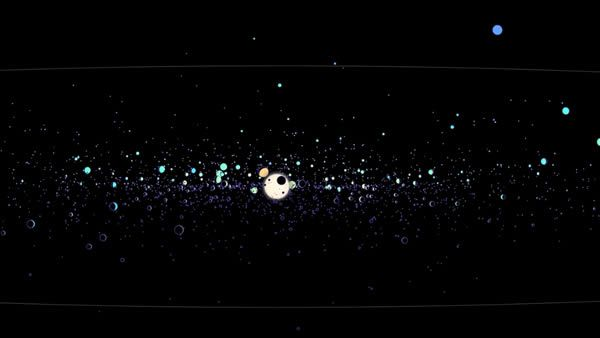
\includegraphics[width=0.8\textwidth]{images/worlds.jpg}
  \caption{Image of Worlds Visualisation}
\end{figure}
This animation is layed out very similarly to the Kepler Visualisation Tool that I am extending. This means that it provides insights into how my visualisation can be improved as Worlds is a much more visually appealing system. By researching how it displays its Exoplanets I can further improve my own visualisation.

\subsection{The Kepler Orrery and The Kepler Orrery 2 - Non interactive}
The Kepler Orrery \cite{orrery} illustrates the exoplanet candidates in their own solar systems. The orbit radii are to scale with respect to each other and planet sizes are to scale with respect to each other, but orbits and planet sizes are different scales. The colors are in order of semi-major axis: two-planet systems (242 in all) have a yellow outer planet; 3-planet (85) green, 4-planet (25) light blue, 5-planet (8) dark blue, 6-planet (1, Kepler-11) purple. 
\begin{figure}[h!]
  \centering
      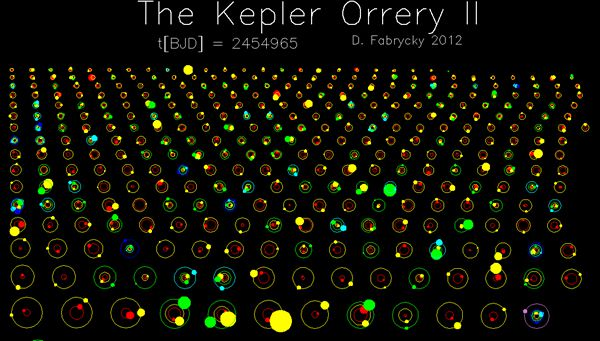
\includegraphics[width=0.8\textwidth]{images/orrery.jpg}
  \caption{Image of The Kepler Orrery Visualisation}
\end{figure}
This system exhibits small multiples, a grid of small similar graphics or charts, allowing them to be easily compared. This provides insights into how I can use small multiples to display information about groups of planets. This will be important for displaying which planets share a solar system.

\subsection{Celestia - Interactive}
Celestia \cite{celestia} is a free real-time space simulation that lets you visually experience the universe in three dimensions. It is an open source system written in C++. 
\begin{figure}[h!]
  \centering
      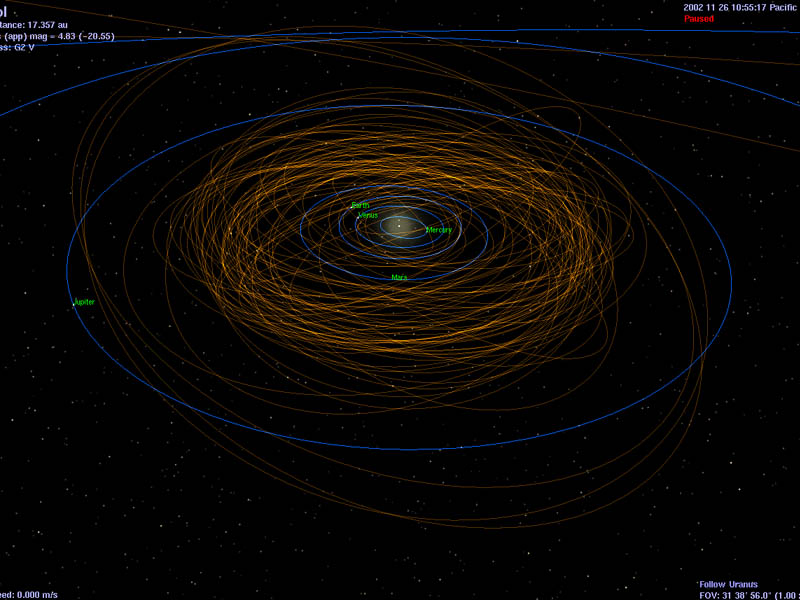
\includegraphics[width=0.5\textwidth]{images/celestia.jpg}
  \caption{Image of Celestia Visualisation}
\end{figure}
This visualisation is much larger and more encompassing system than is needed for this project, as it is a full 3D space simulation. However is does offer insights into how to effectively portray planets and their orbits (See Figure 2.3). It also provides textures that can be used in my visualisation to depict what planets actually look like to increase user immersion.

\subsection{Kepler Visualisation Tool}
An existing system built with Processing is the Kepler Visualisation Tool\cite{kepler_github, kepler_article}. It is a simple visualisation focusing on displaying the candidate Exoplanets temperatures and their locations in relation to their distance from their nearest star, so that a sense of scale can be perceived. Each candidate’s estimated size, orbital speed, and orbital separation is accurately depicted, and each planet is color-coded according to its estimated effective temperature.
\begin{figure}[h!]
  \centering
      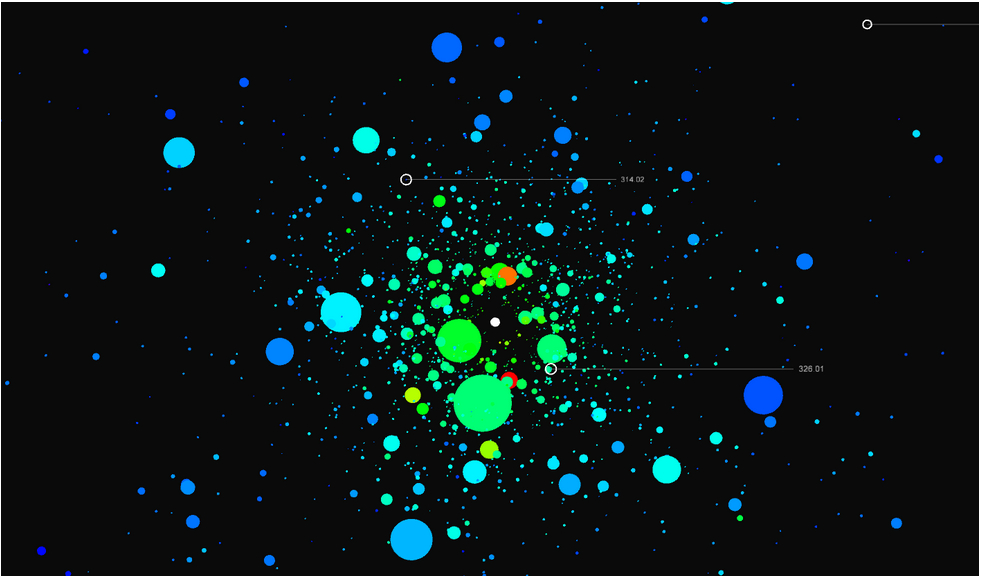
\includegraphics[width=0.8\textwidth]{images/kepler_orbital.jpg}
  \caption{Kepler Visualisation Tool Orbital View}
\end{figure}
\begin{figure}[h!]
  \centering
      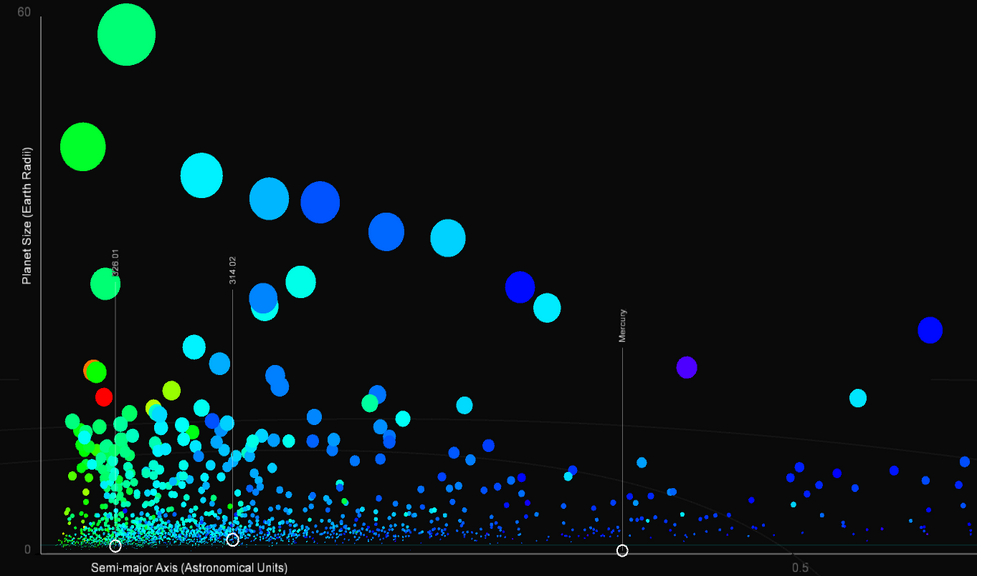
\includegraphics[width=0.8\textwidth]{images/kepler_graph.jpg}
  \caption{Kepler Visualisation Tool Graph View}
\end{figure}
The existing work in this system would serve as foundation for this project. Because much of the visual aspects, and initial data manipulation of the existing system are already complete. It means that implementing the features needed for this projects completion could be focused on more heavily and larger improvements to the existing system can be undertaken, such as better labeling and information displays and user interaction methods.